\documentclass[a1paper,25pt]{tikzposter}

\usepackage[T1]{fontenc}
\usepackage[utf8]{inputenc}
\usepackage[french]{babel}
\usepackage{lmodern}
\usepackage{graphicx}
\usepackage{booktabs}
\usepackage{tabularx}
\usepackage{amsmath}
\usepackage{xcolor}
\usepackage{tikz}

\graphicspath{
  {../rapport/images/}
  {../rapport/diagrams/}
  {../rapport/assets/}
  {../cahier_des_charges/}
  {../preview/}
}

% ============================================================
% COULEURS
% ============================================================
\definecolor{heigred}{HTML}{D0002B}
\definecolor{deepblue}{HTML}{17324D}
\definecolor{softblue}{HTML}{E8F1F8}
\definecolor{softred}{HTML}{FBE9ED}
\definecolor{softgreen}{HTML}{E8F5EE}
\definecolor{textgray}{HTML}{333333}
\definecolor{mutedgray}{HTML}{6B7280}
\definecolor{linegray}{HTML}{D7DEE8}
\definecolor{lasergreen}{HTML}{1F9D55}

% ============================================================
% THEME
% ============================================================
\usetheme{Default}

% Image de fond couvrant toute la page + overlay sombre
\definebackgroundstyle{ImageBG}{
  \node[inner sep=0pt, anchor=center] at (0,0) {%
    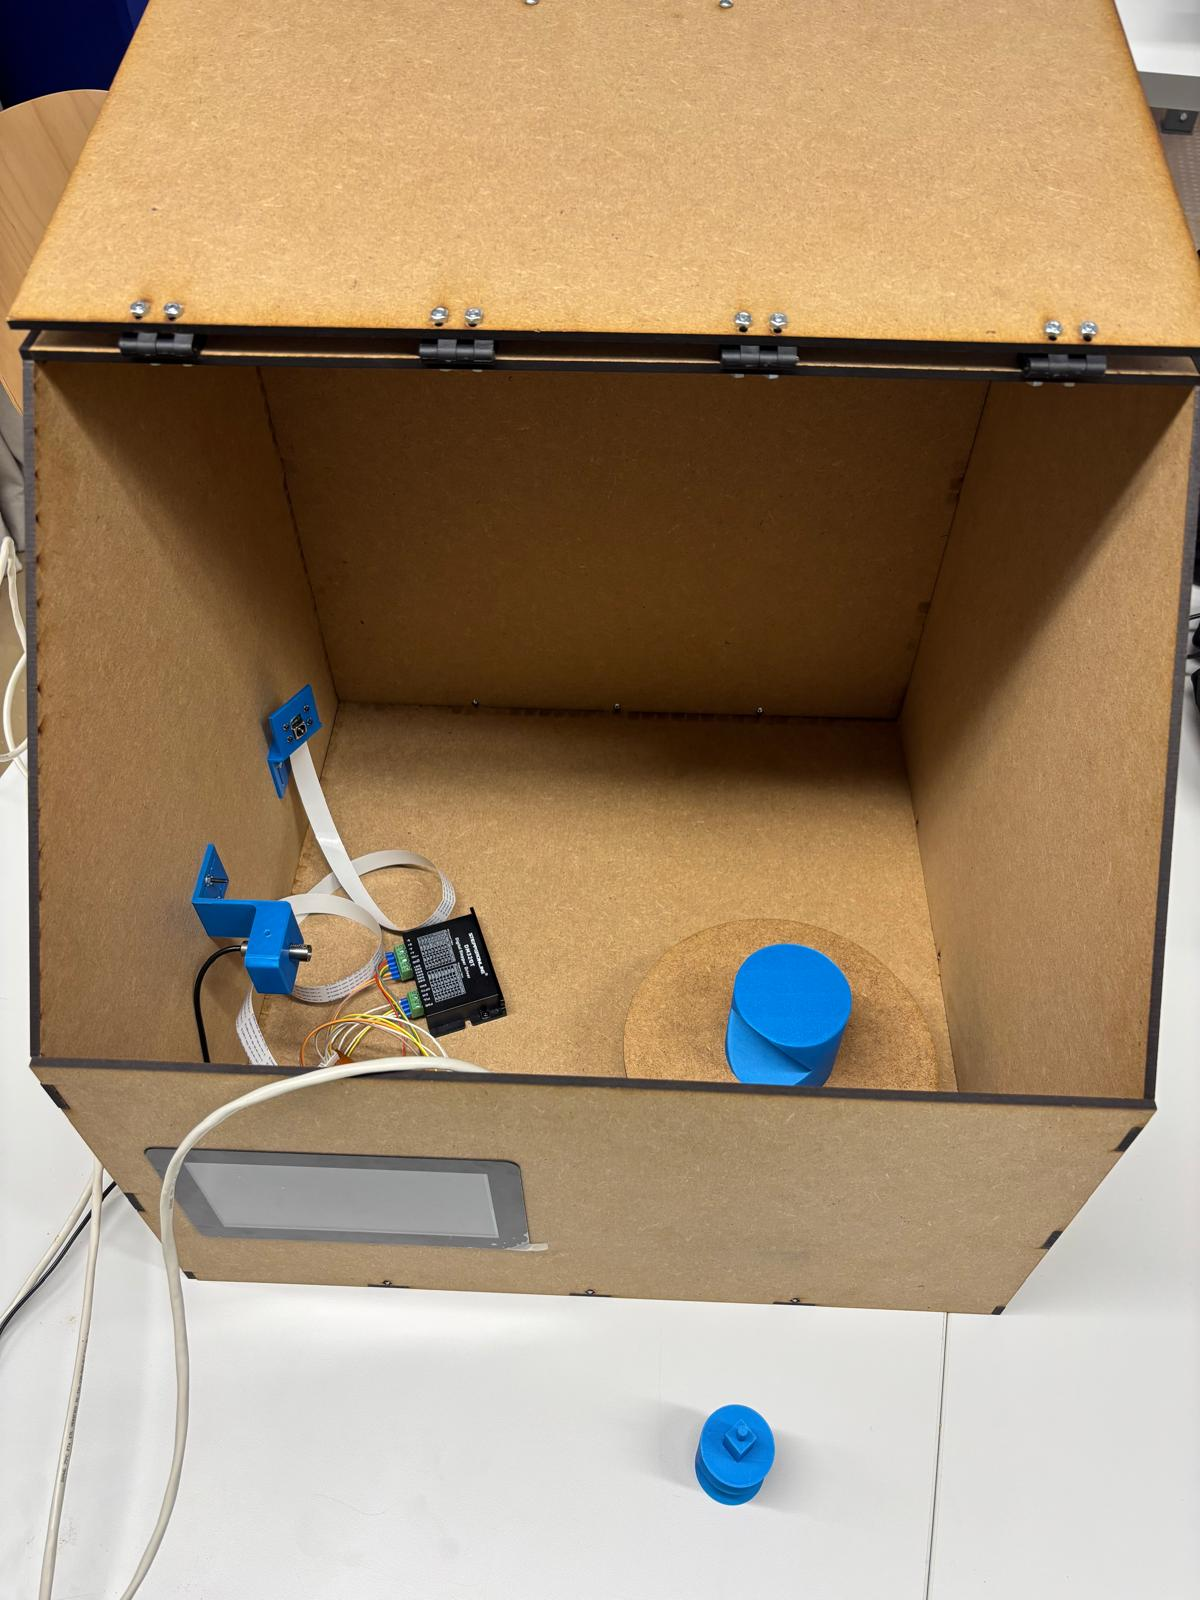
\includegraphics[width=\paperwidth, height=\paperheight]{boite_vue_ext_ouverte.jpeg}%
  };
  \fill[deepblue, opacity=0.80]
    (-0.5\paperwidth,-0.5\paperheight) rectangle (0.5\paperwidth,0.5\paperheight);
}
\usebackgroundstyle{ImageBG}

\definecolorstyle{ScannerStyle}{
  \definecolor{colorOne}{named}{deepblue}
  \definecolor{colorTwo}{named}{heigred}
  \definecolor{colorThree}{named}{softblue}
}{
  \colorlet{backgroundcolor}{deepblue}
  \colorlet{framecolor}{deepblue!60!black}
  \colorlet{titlefgcolor}{white}
  \colorlet{titlebgcolor}{deepblue}
  \colorlet{blocktitlebgcolor}{deepblue}
  \colorlet{blocktitlefgcolor}{white}
  \colorlet{blockbodybgcolor}{white}
  \colorlet{blockbodyfgcolor}{textgray}
  \colorlet{innerblocktitlebgcolor}{softblue}
  \colorlet{innerblocktitlefgcolor}{deepblue}
  \colorlet{innerblockbodybgcolor}{white}
  \colorlet{innerblockbodyfgcolor}{textgray}
}
\usecolorstyle{ScannerStyle}

\defineblockstyle{GlassBlock}{
  titlewidthscale=1.0,
  bodywidthscale=1.0,
  titlecenter,
  titleoffsetx=0pt,
  titleoffsety=0pt,
  bodyoffsetx=0pt,
  bodyoffsety=0pt,
  bodyverticalshift=0pt,
  roundedcorners=12,
  linewidth=0pt,
  titleinnersep=12pt,
  bodyinnersep=16pt
}{
  \fill[blocktitlebgcolor, opacity=0.95, rounded corners=\blockroundedcorners]
    (blocktitle.south west) rectangle (blocktitle.north east);
  \fill[white, opacity=0.94, rounded corners=\blockroundedcorners]
    (blockbody.south west) rectangle (blockbody.north east);
}
\useblockstyle{GlassBlock}

% Titre
\definetitlestyle{ScannerTitle}{
  width=0.93\paperwidth,
  roundedcorners=14,
  linewidth=0pt,
  innersep=14pt,
  titletotopverticalspace=12mm,
  titletoblockverticalspace=16mm
}{
  \fill[deepblue!95!black, opacity=0.95, rounded corners=\titleroundedcorners]
    (\titleposleft,\titleposbottom) rectangle (\titleposright,\titlepostop);
  \draw[heigred, line width=3pt]
    (\titleposleft+0.5cm, \titleposbottom) -- (\titleposleft+5cm, \titleposbottom);
  \draw[white!50, line width=2pt]
    (\titleposleft+5.3cm, \titleposbottom) -- (\titleposright-0.5cm, \titleposbottom);
}
\usetitlestyle{ScannerTitle}

% Supprimer le logo tikzposter en bas
\tikzposterlatexaffectionproofoff

% ============================================================
% TITRE
% ============================================================
\title{%
  \parbox{0.70\textwidth}{%
    \centering
    {\VERYHuge\bfseries\color{white} Scanner 3D \`{a} triangulation laser}\\[0.4cm]
    {\LARGE\color{white!80} Projet multidisciplinaire -- HEIG-VD 2026}\\[0.3cm]
    {\large\color{white!65} L.~Marchand \quad T.~Stamm \quad J.~Weber \quad H.~Fuentes \quad T.~Berthoud}
  }%
}
\author{}
\institute{}

\begin{document}

\maketitle

% Logos places en absolus sur le bandeau titre
\node[anchor=west, inner sep=0pt] at (-0.42\paperwidth, 0.5\paperheight-7cm) {%
  
\includegraphics[height=4cm]{logo_heig.png}%
};
\node[anchor=east, inner sep=0pt] at (0.42\paperwidth, 0.5\paperheight-7cm) {%
  
\includegraphics[height=4cm]{logo_hesso.pdf}%
};

% ============================================================
% RANGEE 1 : LE PROJET + PIPELINE
% ============================================================
\begin{columns}

\column{0.48}
\block{Le projet}{
  {\Large\bfseries\textcolor{deepblue}{Num\'{e}riser un objet physique en fichier 3D imprimable}}\\[0.6cm]
  {\large
  Scanner 3D open-source con\c{c}u pour le \textbf{MakeLab} de la HEIG-VD.
  Un laser ligne vert (520\,nm) \'{e}claire l'objet pos\'{e} sur un plateau tournant motoris\'{e}.
  Une ou deux cam\'{e}ras capturent le profil d\'{e}form\'{e} de la ligne laser.
  Le logiciel reconstruit un nuage de points 3D et exporte un fichier \textbf{STL} ou \textbf{OBJ},
  directement utilisable pour l'impression 3D ou la visualisation.}

  \vspace{0.8cm}
  \centering
  \colorbox{softgreen}{\parbox{0.90\linewidth}{\centering\Large\bfseries\textcolor{deepblue}{%
    Scan en $\sim$1,5 min ~$\bullet$~ Budget $\leq$ 300 CHF\\[0.2cm]
    Interface web ~$\bullet$~ Open-source
  }}}
  \vspace{0.3cm}
}

\column{0.48}
\block{Pipeline de traitement}{
  \begin{minipage}[c]{0.46\linewidth}
    \centering
    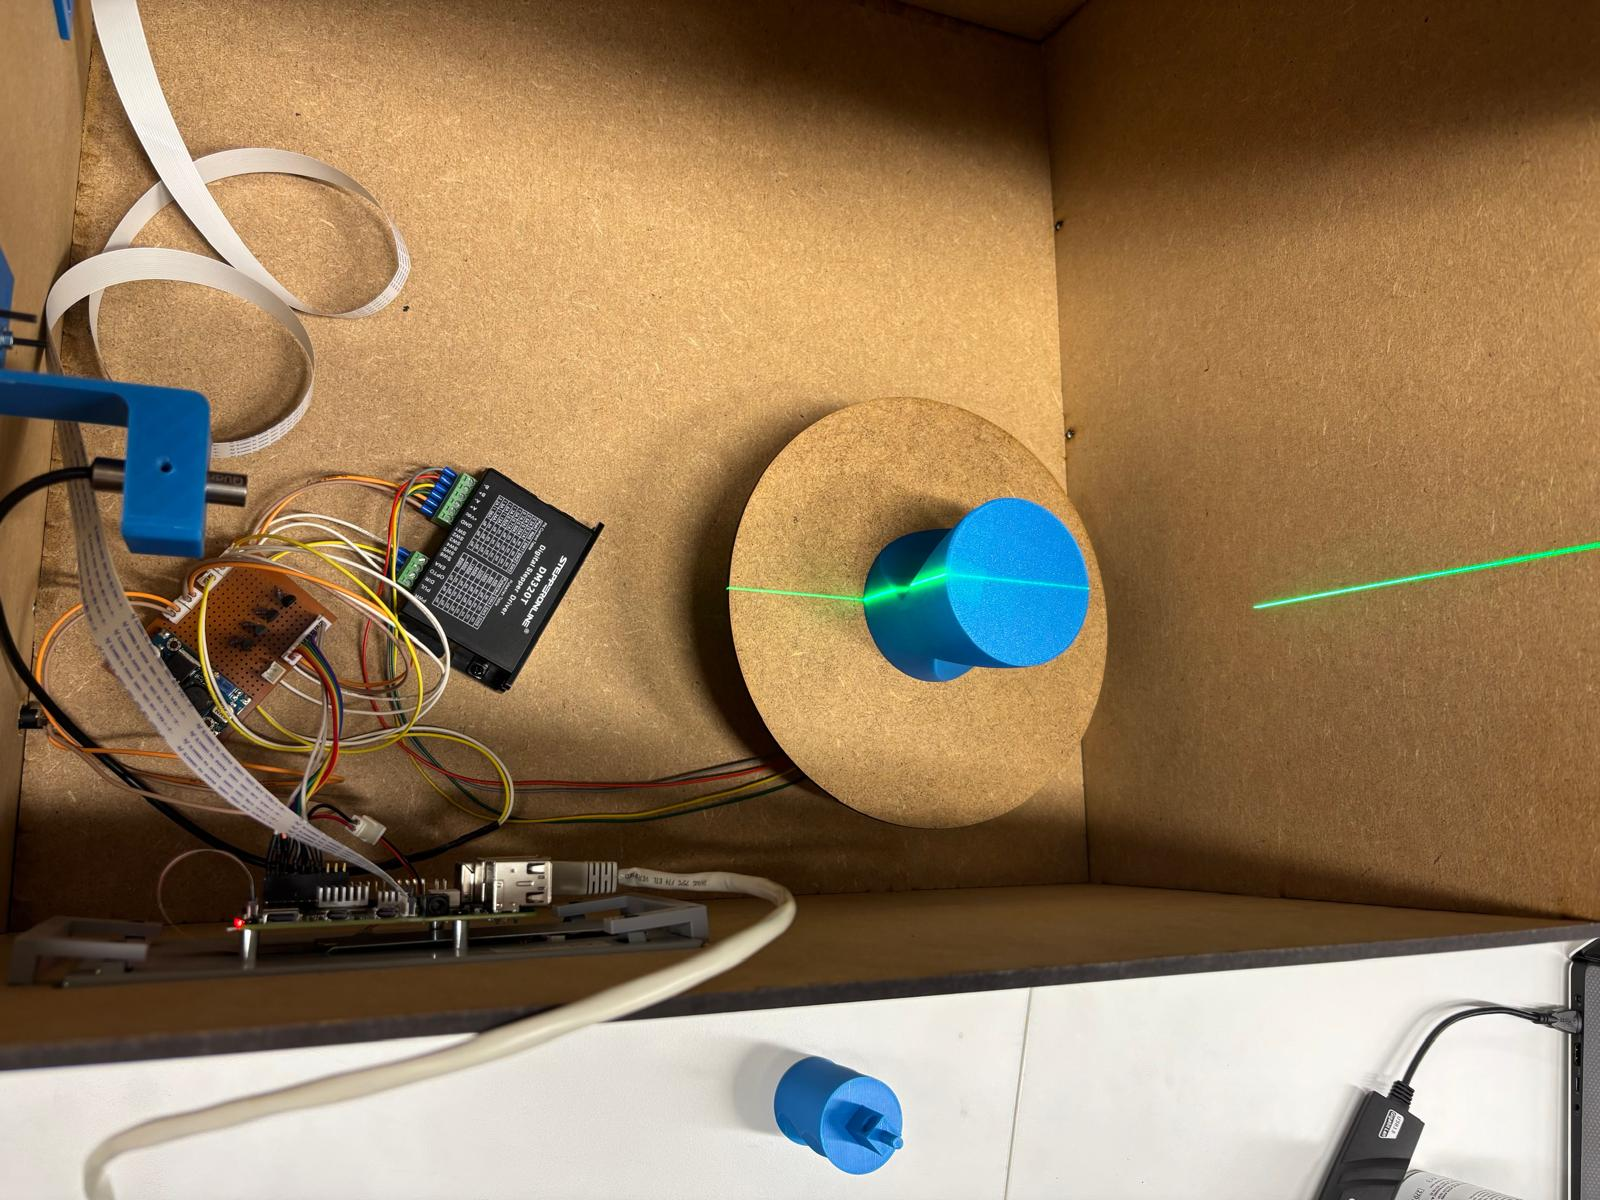
\includegraphics[width=\linewidth,height=10cm,keepaspectratio]{vue_interieur_laser_piece.jpeg}\\[0.3cm]
    {\large Laser sur la pi\`{e}ce}
  \end{minipage}%
  \hfill
  \begin{minipage}[c]{0.46\linewidth}
    \centering
    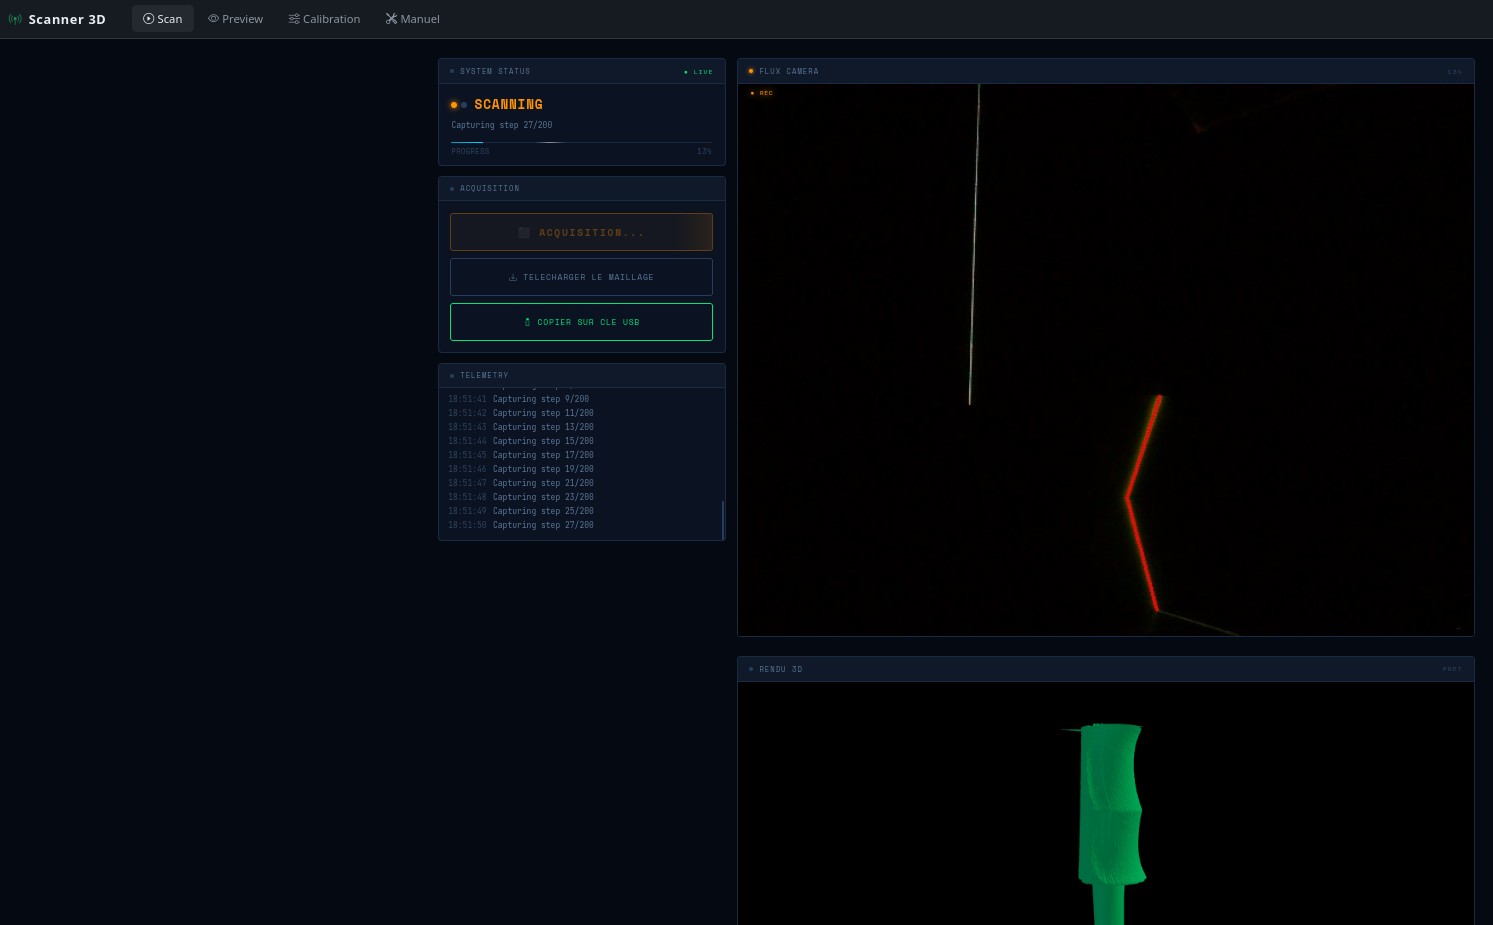
\includegraphics[width=\linewidth,height=10cm,keepaspectratio]{screen_interface.png}\\[0.3cm]
    {\large Interface web + viewer 3D}
  \end{minipage}

  \vspace{0.7cm}
  \centering
  {\Large
  \colorbox{softblue}{\;\textbf{Capture}\;} $\;\rightarrow\;$
  \colorbox{softblue}{\;\textbf{Extraction}\;} $\;\rightarrow\;$
  \colorbox{softblue}{\;\textbf{Triangulation}\;}\\[0.4cm]
  $\rightarrow\;$
  \colorbox{softblue}{\;\textbf{Reconstruction}\;} $\;\rightarrow\;$
  \colorbox{softgreen}{\;\textbf{STL / OBJ}\;}
  }
  \vspace{0.3cm}
}

\end{columns}

% ============================================================
% RANGEE 2 : RESULTATS + DOUBLE CAMERA
% ============================================================
\begin{columns}

\column{0.48}
\block{R\'{e}sultats}{
  \begin{minipage}[t]{0.46\linewidth}
    \centering
    {\Large\bfseries\textcolor{deepblue}{Cylindre}}\\[0.4cm]
    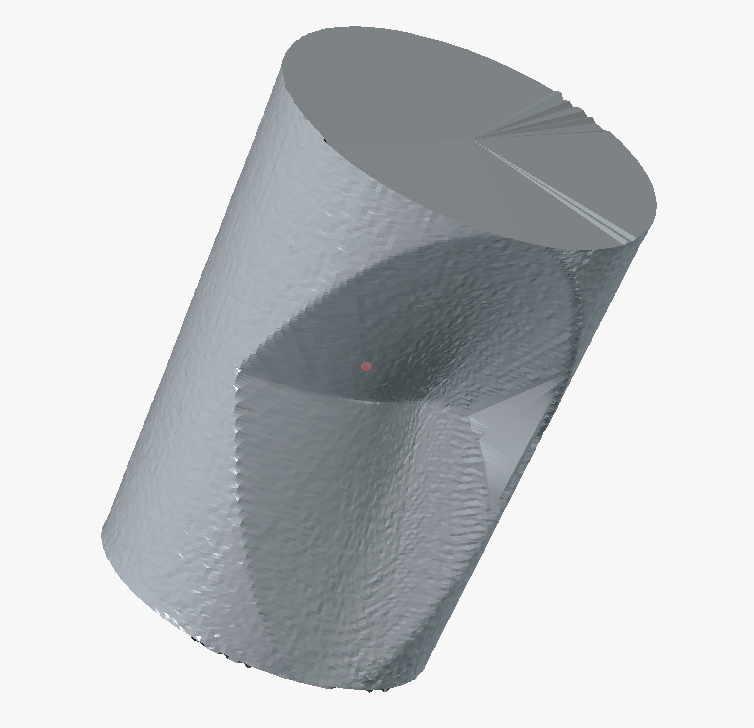
\includegraphics[width=\linewidth,height=10cm,keepaspectratio]{screen_cylindre_stl.png}\\[0.3cm]
    \colorbox{softgreen}{\parbox{0.88\linewidth}{\centering\large\textcolor{deepblue}{\textbf{Forme compl\`{e}te et exploitable}}}}
  \end{minipage}%
  \hfill
  \begin{minipage}[t]{0.46\linewidth}
    \centering
    {\Large\bfseries\textcolor{heigred}{Cube}}\\[0.4cm]
    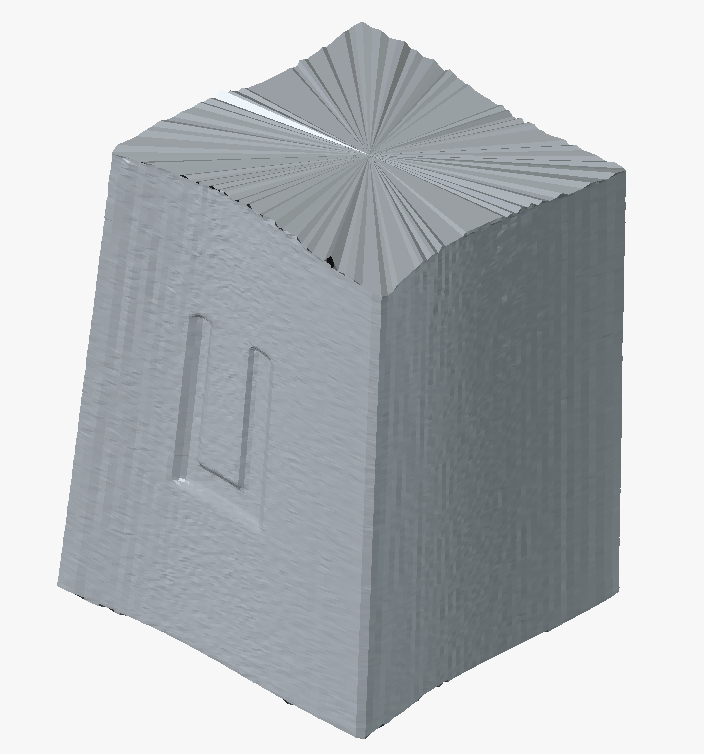
\includegraphics[width=\linewidth,height=10cm,keepaspectratio]{carre_gris_stl.png}\\[0.3cm]
    \colorbox{softred}{\parbox{0.88\linewidth}{\centering\large\textcolor{heigred}{\textbf{Zones masqu\'{e}es par occultation}}}}
  \end{minipage}

  \vspace{0.7cm}
  \begin{center}
  \begin{tikzpicture}
    \node[
      draw=lasergreen, dashed, line width=2pt,
      rounded corners=6pt, fill=softgreen,
      minimum width=0.90\linewidth, minimum height=4cm,
      align=center, text width=0.82\linewidth, inner sep=10pt
    ] {
      {\Large\bfseries\textcolor{deepblue}{R\'{e}sultat double cam\'{e}ra \`{a} ajouter}}\\[0.2cm]
      {\large Comparatif mono vs double sur m\^{e}me pi\`{e}ce}
    };
  \end{tikzpicture}
  \end{center}
}

\column{0.48}
\block{Double cam\'{e}ra}{
  \begin{minipage}[t]{0.46\linewidth}
    \centering
    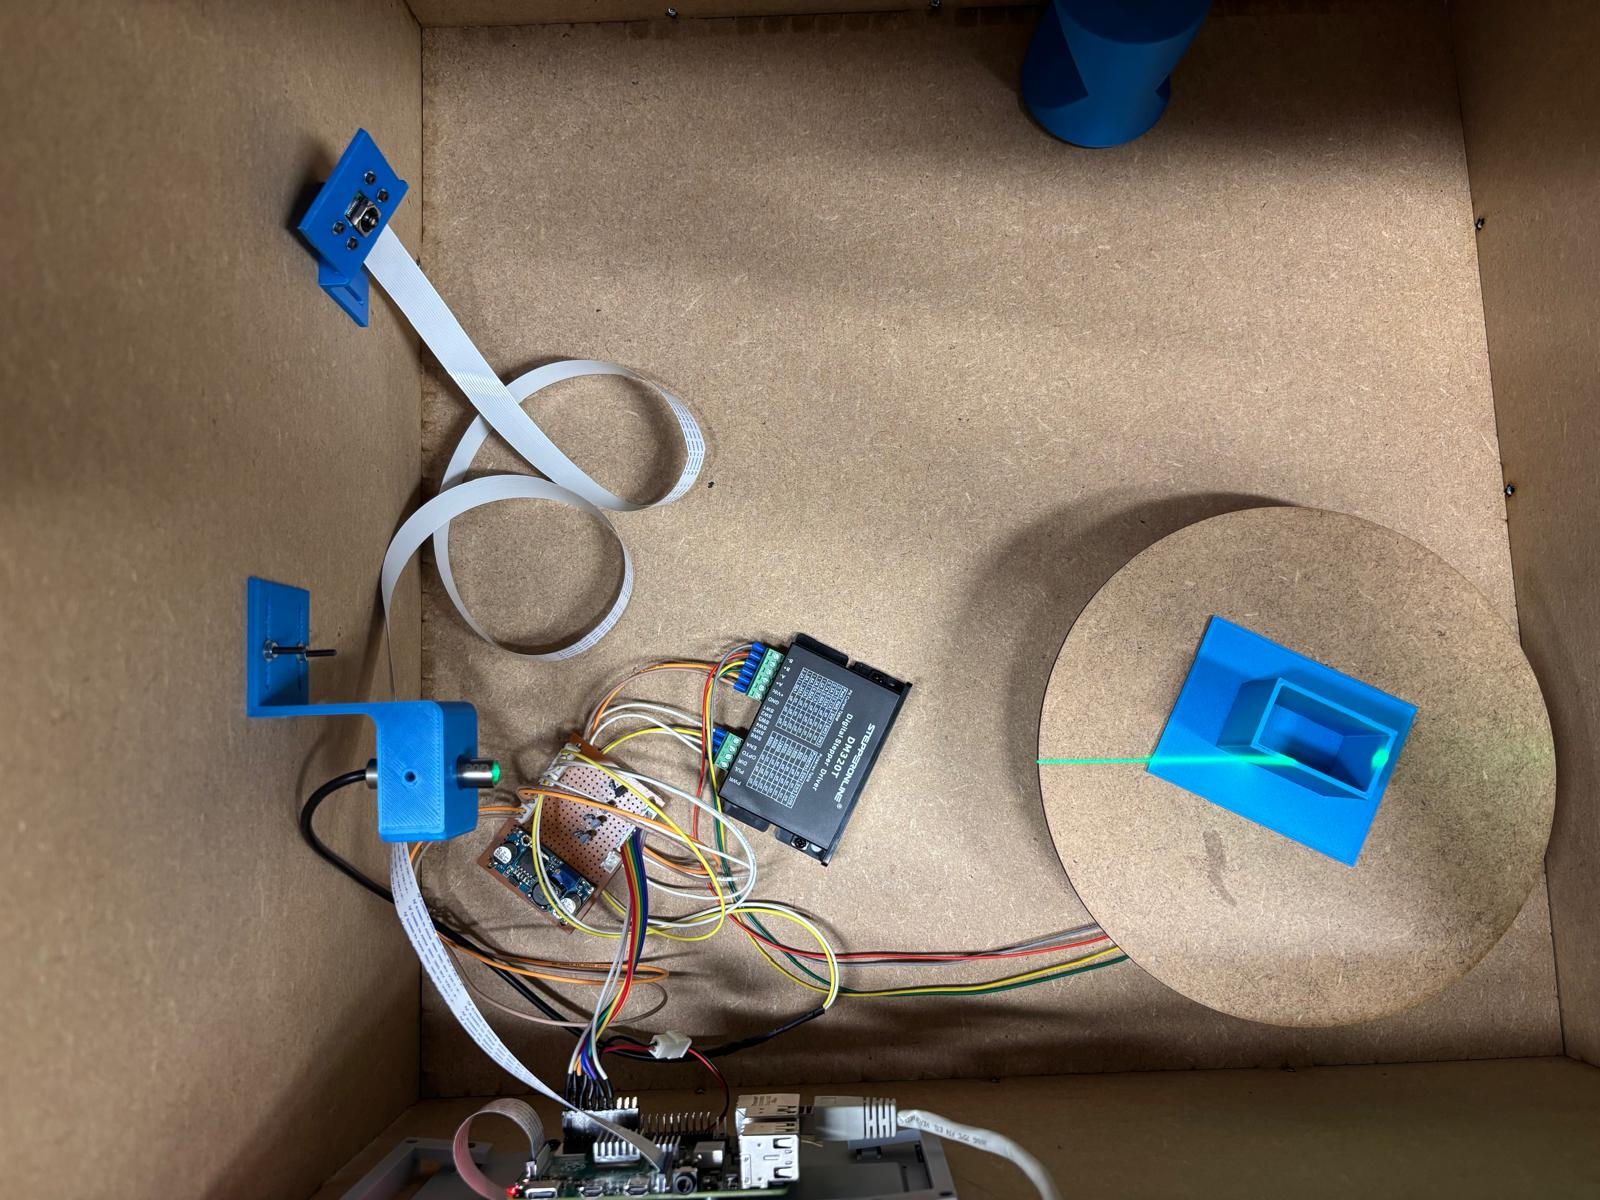
\includegraphics[width=\linewidth,height=10cm,keepaspectratio]{vue_obsturction_laser.jpeg}\\[0.3cm]
    {\large Limite mono-cam\'{e}ra :\\face masqu\'{e}e}
  \end{minipage}%
  \hfill
  \begin{minipage}[t]{0.46\linewidth}
    \centering
    \begin{tikzpicture}
      \node[
        draw=deepblue, dashed, line width=2pt,
        rounded corners=6pt, fill=softblue,
        minimum width=0.90\linewidth, minimum height=10cm,
        align=center, text width=0.80\linewidth, inner sep=10pt
      ] {
        {\Large\bfseries\textcolor{deepblue}{Photo montage}}\\[0.3cm]
        {\large Double cam\'{e}ra install\'{e}e\\dans le prototype}
      };
    \end{tikzpicture}
  \end{minipage}

  \vspace{0.6cm}
  {\Large
  \textbf{Cam\'{e}ra 1} (Pi Camera) : vue haute, $+30^\circ$\\[0.2cm]
  \textbf{Cam\'{e}ra 2} (USB) : vue basse, $-30^\circ$\\[0.4cm]}
  {\large Calibration s\'{e}par\'{e}e par cam\'{e}ra (intrinseques, plan laser, extrinseques).\\
  Fusion des deux nuages dans un rep\`{e}re commun avant export.}
  \vspace{0.2cm}
}

\end{columns}

% ============================================================
% RANGEE 3 : SPECS (barre horizontale compacte)
% ============================================================
\block{Sp\'{e}cifications}{
  \centering
  \vspace{0.2cm}
  {\large
  \renewcommand{\arraystretch}{1.8}
  \begin{tabular}{ccc}
    \colorbox{softblue}{\;\textbf{Temps : $\sim$1,5 min}\;} &
    \colorbox{softblue}{\;\textbf{Objet : $150^3$ mm}\;} &
    \colorbox{softblue}{\;\textbf{Pr\'{e}cision : $\leq$ 2 mm}\;} \\
    \colorbox{softblue}{\;\textbf{Budget : $\leq$ 300 CHF}\;} &
    \colorbox{softblue}{\;\textbf{Export : STL / OBJ}\;} &
    \colorbox{softgreen}{\;\textbf{Python + OpenCV + Open3D}\;}
  \end{tabular}
  }
  \vspace{0.2cm}
}

% ============================================================
% FOOTER
% ============================================================
\node[
  anchor=south,
  minimum width=0.93\paperwidth,
  minimum height=2.5cm,
  fill=deepblue!95!black,
  opacity=0.90,
  rounded corners=10pt,
  inner sep=10pt
] at (0,-0.5\paperheight+3cm) {};

\node[
  anchor=south,
  text=white,
  font=\large
] at (0,-0.5\paperheight+3cm) {%
  HEIG-VD \enspace$\bullet$\enspace D\'{e}partement TIC / TIN
  \enspace$\bullet$\enspace Projet multidisciplinaire PMD 2026
  \enspace$\bullet$\enspace Semestre 4
};

\end{document}
